\chapter{Metodologia}

\section{Problem modeling}
\subsection{General model}
\subsection{Symmetric attenuation}
\subsection{Weak-source regime}
\clearpage
\section{Preprocesamiento}
\subsection{Filtering}
\subsubsection{Filter desing}
\subsection{Normalization}
\subsection{Whitening}
\section{Independent Component Analysis (ICA)}

Independent Component Analysis (ICA) is a fundamental processing technique within Blind Source Separation aimed at recovering latent source signals from observed mixtures without any prior knowledge of the sources or mixing process. As mentioned in previous sections, EMG signals may benefit from this power tool as it allows to decompose multichanel recordings into meaningful physiological components, potentially corresponding to muscle and neural sources.

From a signal processing perspective, ICA a

This section introduces the mathematical formulation and derivation of ICA as well as its basic assumptions and principles. Additionally, a widely used implementation (FastICA) is described, followed by a discussion of ICA's challenges and limitations.
\subsection{Problem formulation}
ICA is originally formulated for linear and instananeous mixing models. Let $s(t)=[s_1(t),...,s_n(t)]$ be an array of stastiscally independent source signals and $x(t)=[x_1(t),...,x_n(t)$ the recorded mixtures. The relationship between both is then given by:

\begin{equation}
    x(t)=As(t)+n(t)
\end{equation}


\subsection{Assumptions of ICA}
Before jumping into mathematical derivations. 
\subsection{ICA derivation (2D)}
\begin{figure}[htbp]
    \centering
    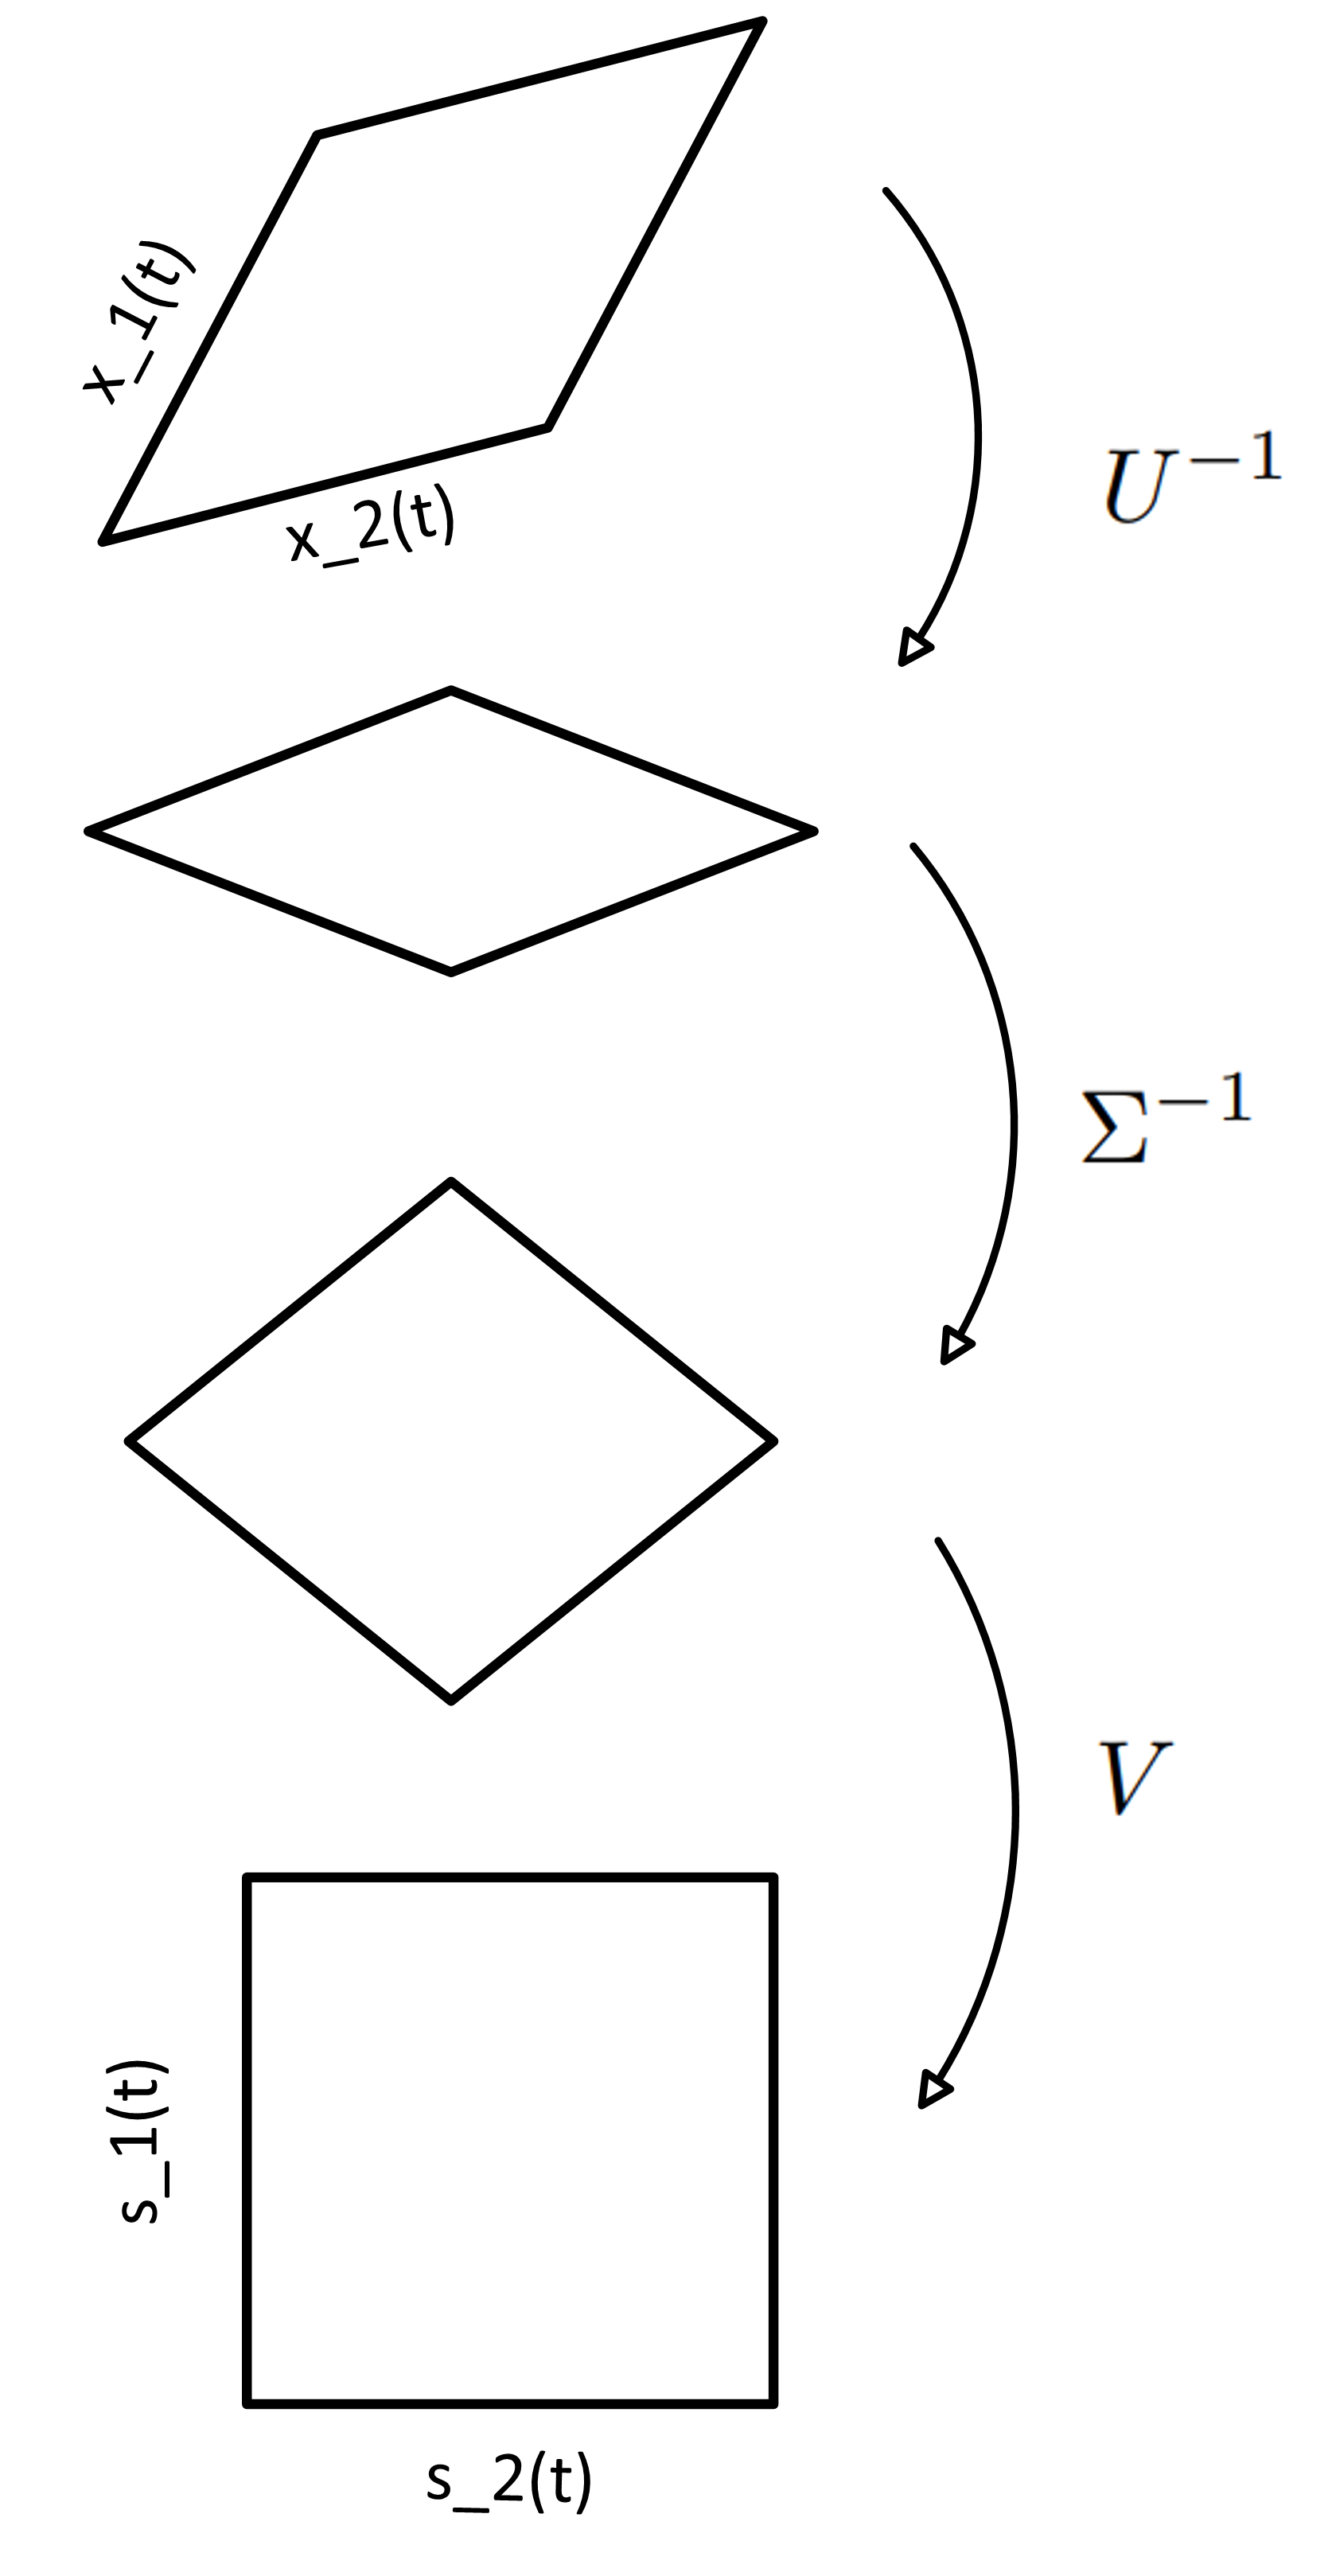
\includegraphics[width=0.5\textwidth]{figuras/ICA_geometry.png}
    \caption{Geometric interpretation of ICA in the 2D case. The observed mixtures are first decorrelated and normalized through whitening (PCA + variance normalization), transforming the data distribution into a spherical shape. The remaining transformation corresponds to a rotation that recovers statistically independent components.}
    \label{fig:ica_whitening}
\end{figure}

\subsection{Implementations: FastICA}
\subsection{Weak-source and noise}
\section{Second-Order Blind Identification (SOBI)}
\section{Constrained(ICA)}
\subsection{Possible constraints}
\subsection{Implementation}
\subsection{Avantages and limitations}
\section{Convolutive / Frequency-domain ICA}
\section{Framework}
\section{Implementacion en vivo}